\chapter{Active learning}
\label{chapter:activelearning}

In this chapter we experiment with the idea of decreasing the number of images needed to
be labeled for training. We present various methods for sampling batches of images in order
to make the training and labeling processes more efficient.

\section{Motivation}
\label{sec:almotivation}

\begin{figure}[!h]
	\centerline{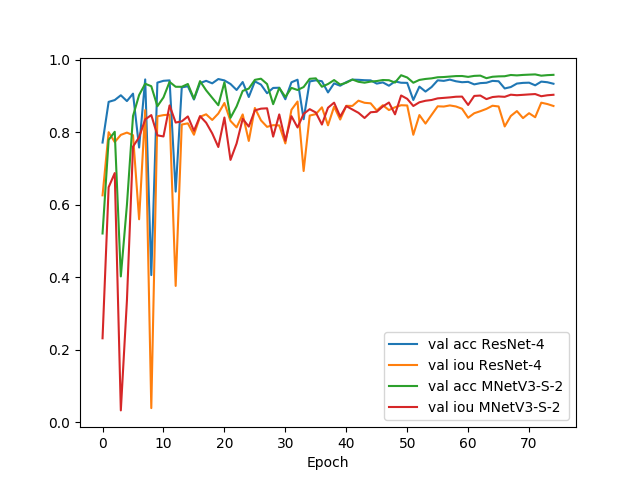
\includegraphics[width=0.8\textwidth]{images/al_random_demonstration.png}}
	\caption[Active learning experiment with random sampling]{Active learning experiment with random sampling. Started with 30 random images and sampling 10 randomly in each round. Three epochs
	are executed within each round. Models: ResNet-4 and MNetV3-S-2. Y-axis represents IoU.}
	\label{img:al_random_initial}
\end{figure}

Each RoboTour contest is held annually in different locations. That means the environment always
changes and datasets gathered and labeled at previous parks might not be sufficient. Creating
new dataset does not only involve capturing images, but also labeling them in order to
produce ground truths for our model. Since labeling entire dataset of images is often an expensive
and time consuming process, we might ask if it is possible to label just a smaller portion of them
and reach comparable accuracy.

\textit{Active learning} may help us in such a situation. The key idea is to label a very small portion
of images at the beginning and start training the model. At some point, the model asks for next
portion of images to be labeled and continues learning. We may stop the training process once
we think the validation loss has converged enough or some other stopping criterion has been met.

Our first experiment is presented in Figure \ref{img:al_random_initial}. We started training
with 30 random images and add 10 random images in each round. Validation accuracy and IoU converged
after $\sim$ 45 epochs with only half of the training images used. It seems
that this approach may help us in order to spend less time labeling.

We prepared an environment on the same machine with graphics processing unit
where we conducted our previous experiments.
In order to understand if it might be profitable to use active learning for training
our models constrained to small amount of data, we decided to perform active learning
simulations. We utilize \textit{ResNet-4} and Deggendorf dataset in our experiments,
but in Section \ref{sec:ablation_study} we show ablation study in which we compare this
model to the other ones.

\section{Random sampling}
\label{sec:random_sampling}

\begin{table}[h]
	\centering
	\begin{tabular}{|c|c|c|c||c|c|c|c|c|c|c|} 
	\hline
	init & pick & reps & stop & imgs & rnds & eps & val acc & val iou & test acc & test iou \\
	\hline
    30 & 10 &  3 & e-val 20 & 216 & 20 & 59 & 0.9521 & 0.9078 & 0.9316 & \textbf{0.8728} \\
    30 & 10 &  3 & e-val 15 & 190 & 17 & 51 & 0.9536 & 0.9081 & 0.9308 & 0.8716 \\
    30 & 15 &  3 & e-val 15 & 244 & 16 & 47 & 0.9509 & 0.9030 & 0.9278 & 0.8638 \\
    30 &  5 &  3 & e-val 15 &  90 & 13 & 39 & 0.9395 & 0.8852 & 0.9238 & 0.8670 \\
    30 & 10 &  6 & e-val 10 & 100 & 8 & 48 & 0.9472 & 0.9031 & 0.9155 & 0.8486 \\
    30 & 10 & 10 & e-val 10 &  56 & 4 & 36 & 0.9414 & 0.8821 & 0.9103 & 0.8465 \\
    30 & 15 & 10 & e-val 10 &  70 & 4 & 36 & 0.9306 & 0.8848 & 0.9079 & 0.8431 \\
    30 & 20 &  6 & e-val 10 & 150 & 7 & 42 & 0.9493 & 0.9103 & 0.9247 & 0.8647 \\
    60 & 20 &  6 & e-val 10 & 133 & 5 & 28 & 0.9400 & 0.8939 & 0.9187 & 0.8586 \\
	\hline
	\end{tabular}
	\caption[Random sampling results.]{Random sampling results. Average of three separate runs.
	\textit{init}: number of images picked initially. \textit{pick}: number of images picked after each round. \textit{reps}: number of
	epoch in one round. \textit{stop}: stopping condition. \textit{imgs}: number of images
	involved in training. \textit{rnds}: number of rounds in total. \textit{eps}: number of epochs
	in total.}
	\label{tab:random_sampling}
\end{table}

As a baseline, we sample images randomly from training data. We pick a bigger bulk of images
initially and train for several round epochs (\textit{reps}). Next samples are picked afterwards
and also trained for the same number of epochs. Since our validation subset is deemed to be
completely labeled, we are able to monitor validation loss. This information helps us
to stop training sooner with early stopping condition. For example, \textit{e-val 10} means
we stop training if the validation loss did not change in last 10 epochs.

According to results in Table \ref{tab:random_sampling}, the test intersection over union
is lower by $2\%$ on average than training the model on full dataset.

\section{Entropy sampling}
\label{sec:entropy_sampling}

\begin{table}[h]
	\centering
	\begin{tabular}{|c|c|c|c||c|c|c|c|c|c|c|} 
	\hline
	init & pick & reps & stop & imgs & rnds & eps & val acc & val iou & test acc & test iou \\
	\hline
    30 & 10 &  3 & e-val 20
        & \begin{tabular}{@{}c@{}}230 \\ 231 \end{tabular}
        & \begin{tabular}{@{}c@{}}21 \\ 22 \end{tabular}
        & \begin{tabular}{@{}c@{}}64 \\ 65 \end{tabular}
        & \begin{tabular}{@{}c@{}}0.9529 \\ 0.9553 \end{tabular}
        & \begin{tabular}{@{}c@{}}0.9114 \\ 0.9089 \end{tabular}
        & \begin{tabular}{@{}c@{}}0.9320 \\ 0.9331 \end{tabular}
        & \begin{tabular}{@{}c@{}}0.8755 \\ 0.8782 \end{tabular} \\
    \hline

    30 & 10 &  3 & e-val 15
        & \begin{tabular}{@{}c@{}}203 \\ 156 \end{tabular}
        & \begin{tabular}{@{}c@{}}18 \\ 14 \end{tabular}
        & \begin{tabular}{@{}c@{}}55 \\ 41 \end{tabular}
        & \begin{tabular}{@{}c@{}}0.9538 \\ 0.9490 \end{tabular}
        & \begin{tabular}{@{}c@{}}0.9133 \\ 0.8993 \end{tabular}
        & \begin{tabular}{@{}c@{}}0.9280 \\ 0.9273 \end{tabular}
        & \begin{tabular}{@{}c@{}}0.8688 \\ 0.8691 \end{tabular} \\
    \hline

    30 & 15 &  3 & e-val 15
        & \begin{tabular}{@{}c@{}}262 \\ 252 \end{tabular}
        & \begin{tabular}{@{}c@{}}17 \\ 16 \end{tabular}
        & \begin{tabular}{@{}c@{}}51 \\ 48 \end{tabular}
        & \begin{tabular}{@{}c@{}}0.9575 \\ 0.9529 \end{tabular}
        & \begin{tabular}{@{}c@{}}0.9151 \\ 0.9047 \end{tabular}
        & \begin{tabular}{@{}c@{}}0.9375 \\ 0.9338 \end{tabular}
        & \begin{tabular}{@{}c@{}}\textbf{0.8815} \\ 0.8759 \end{tabular} \\
    \hline

    30 &  5 &  3 & e-val 15
        & \begin{tabular}{@{}c@{}}111 \\ 135 \end{tabular}
        & \begin{tabular}{@{}c@{}}17 \\ 22 \end{tabular}
        & \begin{tabular}{@{}c@{}}52 \\ 66 \end{tabular}
        & \begin{tabular}{@{}c@{}}0.9510 \\ 0.9512 \end{tabular}
        & \begin{tabular}{@{}c@{}}0.9071 \\ 0.9107 \end{tabular}
        & \begin{tabular}{@{}c@{}}0.9248 \\ 0.9307 \end{tabular}
        & \begin{tabular}{@{}c@{}}0.8636 \\ 0.8744 \end{tabular} \\
    \hline

    30 & 10 &  6 & e-val 10
        & \begin{tabular}{@{}c@{}}86 \\ 70 \end{tabular}
        & \begin{tabular}{@{}c@{}}7 \\ 5 \end{tabular}
        & \begin{tabular}{@{}c@{}}40 \\ 30 \end{tabular}
        & \begin{tabular}{@{}c@{}}0.9442 \\ 0.9285 \end{tabular}
        & \begin{tabular}{@{}c@{}}0.8978 \\ 0.8830 \end{tabular}
        & \begin{tabular}{@{}c@{}}0.9210 \\ 0.9079 \end{tabular}
        & \begin{tabular}{@{}c@{}}0.8573 \\ 0.8456 \end{tabular} \\
    \hline

    30 & 10 & 10 & e-val 10
        & \begin{tabular}{@{}c@{}}66 \\ 63 \end{tabular}
        & \begin{tabular}{@{}c@{}}5 \\ 4 \end{tabular}
        & \begin{tabular}{@{}c@{}}46 \\ 43 \end{tabular}
        & \begin{tabular}{@{}c@{}}0.9435 \\ 0.9363 \end{tabular}
        & \begin{tabular}{@{}c@{}}0.8931 \\ 0.8858 \end{tabular}
        & \begin{tabular}{@{}c@{}}0.9234 \\ 0.9143 \end{tabular}
        & \begin{tabular}{@{}c@{}}0.8652 \\ 0.8532 \end{tabular} \\
    \hline

    30 & 15 & 10 & e-val 10
        & \begin{tabular}{@{}c@{}}55 \\ 65 \end{tabular}
        & \begin{tabular}{@{}c@{}}3 \\ 3 \end{tabular}
        & \begin{tabular}{@{}c@{}}26 \\ 33 \end{tabular}
        & \begin{tabular}{@{}c@{}}0.9358 \\ 0.9375 \end{tabular}
        & \begin{tabular}{@{}c@{}}0.8861 \\ 0.8847 \end{tabular}
        & \begin{tabular}{@{}c@{}}0.9049 \\ 0.9119 \end{tabular}
        & \begin{tabular}{@{}c@{}}0.8373 \\ 0.8508 \end{tabular} \\
    \hline
    
    30 & 20 &  6 & e-val 10
        & \begin{tabular}{@{}c@{}}123 \\ 116 \end{tabular}
        & \begin{tabular}{@{}c@{}}6 \\ 5 \end{tabular}
        & \begin{tabular}{@{}c@{}}34 \\ 32 \end{tabular}
        & \begin{tabular}{@{}c@{}}0.9479 \\ 0.9441 \end{tabular}
        & \begin{tabular}{@{}c@{}}0.8989 \\ 0.8951 \end{tabular}
        & \begin{tabular}{@{}c@{}}0.9259 \\ 0.9220 \end{tabular}
        & \begin{tabular}{@{}c@{}}0.8678 \\ 0.8625 \end{tabular} \\
    \hline
    
    60 & 20 &  6 & e-val 10
        & \begin{tabular}{@{}c@{}}140 \\ 133 \end{tabular}
        & \begin{tabular}{@{}c@{}}5 \\ 5 \end{tabular}
        & \begin{tabular}{@{}c@{}}30 \\ 28 \end{tabular}
        & \begin{tabular}{@{}c@{}}0.9516 \\ 0.9397 \end{tabular}
        & \begin{tabular}{@{}c@{}}0.9130 \\ 0.8852 \end{tabular}
        & \begin{tabular}{@{}c@{}}0.9305 \\ 0.9211 \end{tabular}
        & \begin{tabular}{@{}c@{}}0.8731 \\ 0.8586 \end{tabular} \\
    \hline
	\end{tabular}
	\caption[Entropy sampling results]{Entropy sampling results. Average of three separate runs.
	The first subrow in each row
	describes results of averaging entropy over pixels and the second subrow describes results
	of summing the entropy.}
	\label{tab:entropy_sampling}
\end{table}

A straightforward way to improve random sampling might be to sample images based on
the level of model's uncertainty predicting them. Before the images are picked, we need
to sort them according to some score. A good candidate seems to be entropy. The output
of the model is a 2D matrix with the same shape like input image, where each cell contains the
number in range from 0 to 1. This number denotes the probability of pixel being driveable.
Therefore, entropy of $i$-th pixel might be computed by the following formula:

$$H_i = -(p_i\log_2(p_i) + (1-p_i)\log_2(1-p_i))$$

where $p_i$ denotes the probability of pixel being driveable. An aggregate function is applied
afterwards to attach single score number to the image. In our case, we use \textit{average} and
\textit{sum}.
Table \ref{tab:entropy_sampling} captures results of both average and sum entropy sampling.
There is no obvious winner between sum and average functions in entropy sampling because
both perform quite similarly. Reducing
the number of epochs for stopping condition to execute also reduces the number of rounds and
images sampled as expected. \textit{e-val 10} seems to be a good candidate for stopping since we
do not end up labeling entire dataset. Batches of 20 images seem to work better in combination
with \textit{e-val 10}.
If we compare these results, we can see that there is a very slight improvement over random sampling.
However, we are able to get nice test IoU with only $50\%$ images of entire dataset, which
makes the labeling process more efficient.

In Figure \ref{img:boxplot_entropy} we demonstrate a simulation of how both entropy and 
validation IoU evolve with each round. Clearly, we can see that at some point the model
does not learn pretty much no new information and the training procedure might be stopped.

\begin{figure}[!h]
	\centerline{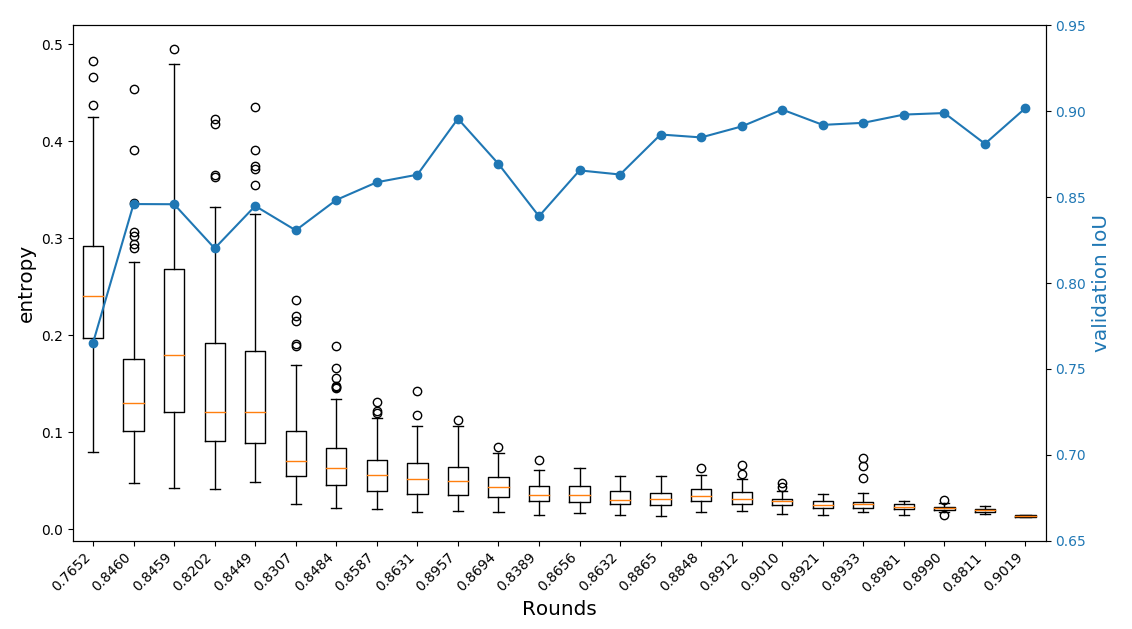
\includegraphics[width=1.05\textwidth]{images/boxplot_entropy.png}}
	\caption[Comparison of entropies and validation IoU]{Comparison of entropies and validation IoU
	in each round. Started with 30 labeled images and within each round we sample 10 images.
	Entropies (averaged over pixels) are computed over all of the unlabeled images.}
	\label{img:boxplot_entropy}
\end{figure}

\section{Diversity sampling}
\label{sec:diversity_sampling}

The problem with entropy (or uncertainty) sampling is that images with highest score
might be in many cases similar and the change will not be as high as expected
\cite{bib:sener2017active, bib:yang2017suggestive, bib:zhdanov2019diverse}.
Therefore, before we actually sample images based on some score, we want to put them
into categories based on their similarity. A good candidate for this task might be
well known \textit{K-means} algorithm described in Section
\ref{sec:image_segmentation:cluster_based}.

Within the model, encoder's role is to produce feature vector, which holds the information
that represent the input. Hence, it is a good candidate to represent the image
when running K-means.
In case of the ResNet-4, the last encoder's layer produces 128 feature maps
with resolution of $15\times 20$. Each cell's value is set to be the average over all of the
feature map's cells and the resulting matrix is flattened into one long vector with
dimension of 300. The number of clusters, which is a hyperparameter in K-means setting,
is set to be the number of images we sample within each round. 

After running K-means from package called \textit{Scikit-learn} \cite{bib:pedregosa2011scikit},
we compute entropies and sample one image with highest entropy per
cluster. Table \ref{tab:diversity_sampling} shows the results of diversity sampling.
It beats both random and entropy sampling. Moreover, results are more consistent so we do not
end up with very low IoU.

\begin{table}[h]
	\centering
	\begin{tabular}{|c|c|c|c||c|c|c|c|c|c|c|} 
	\hline
	init & pick & reps & stop & imgs & rnds & eps & val acc & val iou & test acc & test iou \\
	\hline
    30 & 10 &  3 & e-val 20 & 210 & 19 & 58 & 0.9522 & 0.9127 & 0.9320 & 0.8758 \\
    30 & 10 &  3 & e-val 15 & 210 & 13 & 40 & 0.9486 & 0.9041 & 0.9206 & 0.8550 \\
    30 & 15 &  3 & e-val 15 & 202 & 13 & 38 & 0.9501 & 0.9068 & 0.9213 & 0.8608 \\
    30 &  5 &  3 & e-val 15 & 97 & 14 & 43 & 0.9477 & 0.8995 & 0.9228 & 0.8617 \\
    30 & 10 &  6 & e-val 10 & 83 & 6 & 38 & 0.9441 & 0.8984 & 0.9224 & 0.8629 \\
    30 & 10 & 10 & e-val 10 & 60 & 4 & 40 & 0.9442 & 0.8973 & 0.9168 & 0.8525 \\
    30 & 15 & 10 & e-val 10 & 75 & 4 & 40 & 0.9443 & 0.8934 & 0.9197 & 0.8601 \\
    30 & 20 &  6 & e-val 10 & 143 & 7 & 40 & 0.9517 & 0.9078 & 0.9261 & 0.8644 \\
    60 & 20 &  6 & e-val 10 & 153 & 6 & 34 & 0.9503 & 0.9046 & 0.9306 & \textbf{0.8770} \\
	\hline
	\end{tabular}
	\caption[Diversity sampling results]{Diversity sampling results. Average of three
	separate runs. The \textit{pick} denotes
	the number of clusters as well as the number of images sampled in a round.}
	\label{tab:diversity_sampling}
\end{table}

In order to compare these three aforementioned methods for sampling batches of images,
we ran our experiments without early stopping condition. Three separate runs are conducted
for each method within each experiment and the results are averaged. The results are
presented in Figure \ref{img:method_comparison}. Clearly, both \textit{average entropy} and
\textit{diversity} sampling perform comparably similar and better than the random
sampling, and reach higher accuracy sooner. 
The difference is not very significant, but might help with efficient training in
a setting with lower number of images in dataset. A small difference in IoU with
fully labeled dataset is caused probably by not sufficient number of epochs the
models were trained in last rounds.

\begin{figure}[!h]
	\begin{center}
	    \subfloat[10 samples and 6 epochs per round. ]{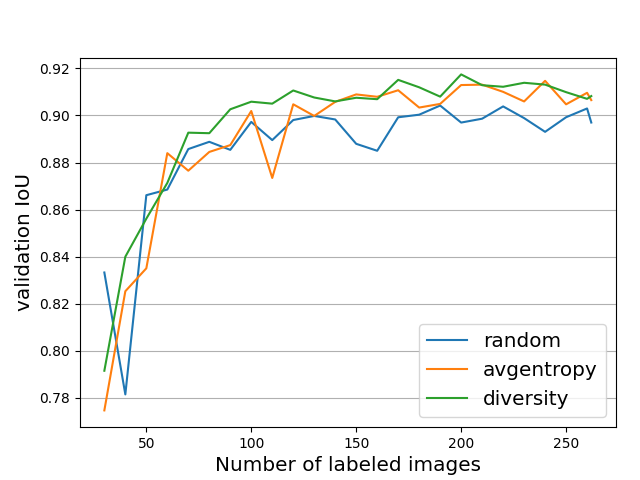
\includegraphics[width=0.54\textwidth]{images/comparison_expA.png}}
		\subfloat[20 samples and 6 epochs per round. ]{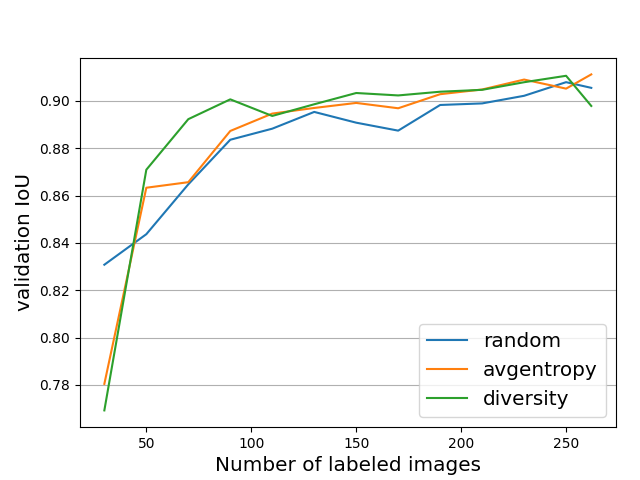
\includegraphics[width=0.54\textwidth]{images/comparison_expB.png}}
		\quad
		\subfloat[15 samples and 10 epochs per round. ]{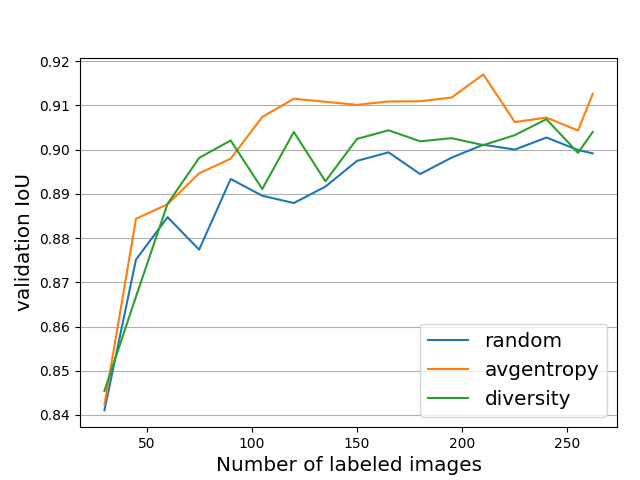
\includegraphics[width=0.54\textwidth]{images/comparison_expC.png}}
	\end{center}
	\caption[Comparison of sampling methods]{Comparison of sampling methods based on three separate experiments.}
	\label{img:method_comparison}
\end{figure}

The initial batch of images is still being sampled randomly, so we would like to
test whether choosing images in this initial batch might be done more wisely. The input
image contains $640\cdot 480 \cdot 3 = 921 600$ pixels. This would be a very high
dimensional vector as an input to K-means and thus dimension reduction is essential in
this case. Recently, \textit{UMAP} \cite{bib:mcinnes2018umap}
(Uniform Manifold Approximation and Projection) algorithm for dimension reduction
has been proposed. It is competitive with \textit{t-SNE} \cite{bib:maaten2008visualizing}
in terms of visualization quality, while preserving more of the global structure
with superior run time performance.

Fortunately, there is UMAP python package \cite{bib:mcinnes2018umap-software} available
for a free usage. All the images available in the train subset are loaded into memory and
normalized to values in the range from 0 to 1. Channels are subsequently flattened
into one long vector and dimension is reduced by UMAP algorithm. The output is then
fed to the K-means.

After a couple of experiments with UMAP, we found out that in our case of such a small
dataset, there is no improvement at all, since such a small portion of initial images
does not affect the overall efficiency.

\section{Ablation study}
\label{sec:ablation_study}

Experiments in sections above are conducted with ResNet-4 minimized model. 
In this Section, we test MNetV3-S-2 and SNetV2-1 in active learning setting.
We tested both models within four experiments, see Table \ref{tab:ablation_study}.

\begin{table}[!h]
    \begin{tabular}{|c|c|c|c|c||c|c|c|c|c|c|c|}
    \hline
    \rotatebox[origin=c]{90}{ model } & init & pick & reps & stop & imgs & rnds & eps & val acc & val iou & test acc & test iou \\ \hline
    \multirow{4}{*}{\rotatebox[origin=c]{90}{MNetV3-S-2}}
        & 30 & 10 & 6 & e-val 10 & 117 & 10 & 58 & 0.9391 & 0.8912 & 0.9245 & 0.8640 \\ \cline{2-12} 
        & 30 & 15 & 10 & e-val 10 & 125 & 7 & 73 & 0.9439 & 0.8980 & 0.9319 & 0.8704 \\ \cline{2-12} 
        & 30 & 20 & 6 & e-val 10 & 183 & 26 & 52 & 0.9449 & 0.9044 & 0.9231 & 0.8668 \\ \cline{2-12} 
        & 60 & 20 & 6 & e-val 10 & 227 & 9 & 56 & 0.9535 & 0.9131 & 0.9394 & \textbf{0.8799} \\ \hline\hline
    \multirow{4}{*}{\rotatebox[origin=c]{90}{SNetV2-1}}
        & 30 & 10 & 6 & e-val 10 & 123 & 10 & 62 & 0.9475 & 0.9046 & 0.9298 & 0.8680 \\ \cline{2-12} 
        & 30 & 15 & 10 & e-val 10 & 135 & 8 & 80 & 0.9521 & 0.9114 & 0.9351 & 0.8772 \\ \cline{2-12}
        & 30 & 20 & 6 & e-val 10 & 197 & 9 & 56 & 0.9476 & 0.8943 & 0.9381 & 0.8799 \\ \cline{2-12} 
        & 60 & 20 & 6 & e-val 10 & 234 & 10 & 60 & 0.9506 & 0.9079 & 0.9398 & \textbf{0.8805} \\ \hline
    \end{tabular}
    \caption[Results of MNetV3-S-2 and SNetV2-1 in active learning setting]{Results of MNetV3-S-2 and SNetV2-1 in active learning setting. Average of three separate runs. For clarification of the header see Table \ref{tab:random_sampling}.}
    \label{tab:ablation_study}
\end{table}

The results of both models are comparably similar to the ResNet-4.
The only significant change can be seen in the second row where the model uses much less data
and performs good enough. The mobile models make use of more images on average. That might be
caused by the number of parameters, which is almost four times higher and the early stopping
condition is met later because the models still manage to update some of their weights,
leading to slightly better accuracy.

